\documentclass[11pt,a4paper]{article}
\usepackage{ctex}
\usepackage[utf8]{inputenc}
\usepackage{geometry}
\usepackage{fancyhdr}
\usepackage{enumitem}
\usepackage{titlesec}
\usepackage{amsmath} % Added for math equation support
\usepackage{amssymb}
\usepackage{graphicx} % Added for including graphics
\usepackage{titling}
\usepackage{subcaption}

\usepackage{multicol}
\usepackage{listings}
\usepackage{booktabs}
\usepackage{multirow}

\usepackage[hidelinks]{hyperref}
% \usepackage[style=authoryear]{biblatex} % Use biber backend
% \addbibresource{../../paper.bib} % Specify the .bib file
% Define \lll

\geometry{margin=0.5in}
\titleformat{\section}{\large\bfseries}{\thesection}{0.5em}{}

% title context and style setting
\title{周报-向嘉豪(2024-12-09)}
\setlength{\droptitle}{-6em} % Reduce space begin the title
% Redefine \maketitle to display only the title
\renewcommand{\maketitle}{
  \begin{center}
    \LARGE\bfseries\thetitle
  \end{center}
}

\begin{document}

\maketitle


\noindent \textbf{Abstract}: 本周工作主要聚焦于论文的最终修订与投稿准备工作。在论文修订方面,我们完成了以下工作:1)通过引入amssymb数学符号库,规范了全文的数学公式与符号体系;2)完善了参考文献的基础信息,确保符合IEEE引用规范。在投稿准备方面:1)基于IEEE计算机学会出版指南完成了投稿材料准备;2)深入研究IEEE Author Portal系统,熟悉了投稿流程;3)经过审慎考虑,决定将论文投向IEEE Trans. on Computers。

\noindent \textbf{下周计划}: 1)完成IEEE Trans. on Computers的在线投稿


\subsection{论文修订与规范化}

针对IEEE期刊格式要求,我们对论文进行了系统性修订。在符号体系方面,通过引入amssymb数学符号库,解决了特殊数学符号(如$\ggg$)的显示问题。同时,对全文的数学公式和符号进行了统一规范。在文献引用方面,我们完善了所有参考文献的基础信息,包括补充缺失的页码范围和期刊卷号,确保符合IEEE引用规范。

\subsection{投稿准备工作}

基于IEEE计算机学会出版指南(\url{https://www.computer.org/publications/author-resources}),我们完成了投稿材料的系统性准备工作。通过深入研究IEEE Author Portal系统(见图~\ref{fig:authorportal}),我们熟悉了完整的投稿流程,并按要求撰写了投稿信(见图~\ref{fig:coverletter})。考虑到研究内容的性质以及IEEE Trans. on Info. Forensics and Security偏重理论性研究的特点,经老师指导后,决定将论文投向IEEE Trans. on Computers。目前,所有投稿材料均已完备,即将开始投稿程序。
\begin{figure}[h]
  \centering
  \begin{subfigure}[b]{0.2\textwidth}
    \centering
    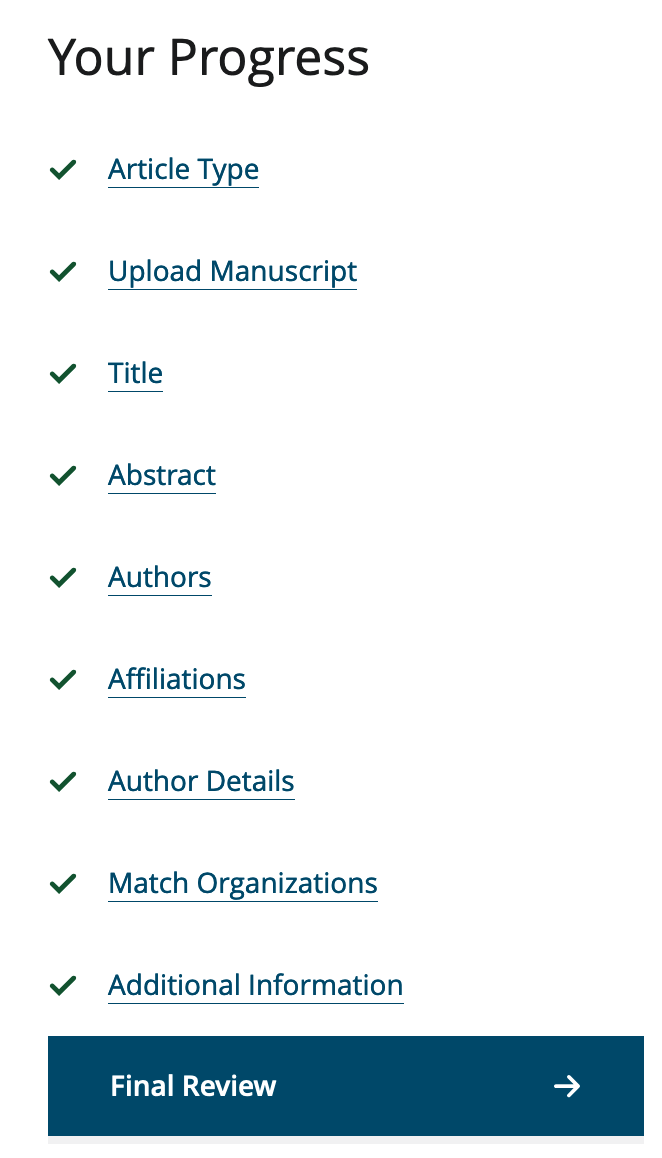
\includegraphics[width=\textwidth]{./fig/submit.png}
    \caption{投稿流程}
    \label{fig:authorportal}
  \end{subfigure}
  \hfill
  \begin{subfigure}[b]{0.48\textwidth}
    \centering
    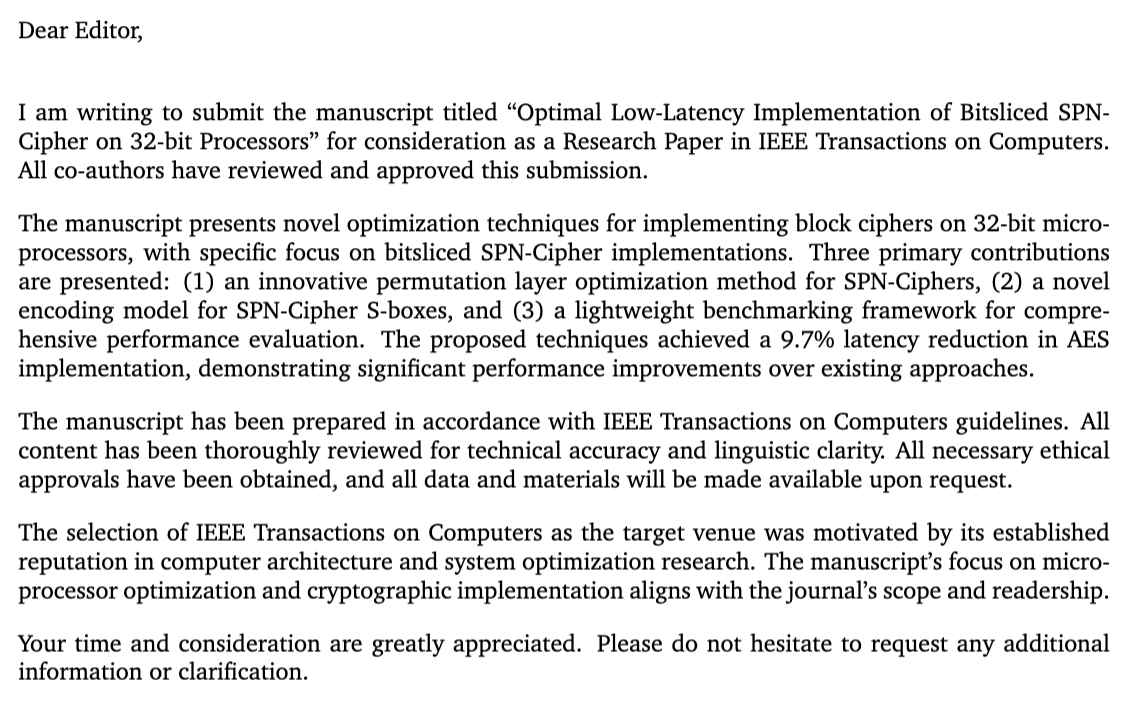
\includegraphics[width=\textwidth]{./fig/CoverLetter.png}
    \caption{投稿cover letter}
    \label{fig:coverletter}
  \end{subfigure}
  \caption{论文投稿材料准备}
  \label{fig:submission_materials}
\end{figure}



% \newpage
% % Add some vertical space to push content to bottom if needed
% \vfill


% % Include the bibliography
% \bibliographystyle{alpha}
% \bibliography{../../paper}

\end{document}